\documentclass[a4paper, 10pt, conference]{ieeeconf}

\IEEEoverridecommandlockouts

\usepackage[a4paper, top=54pt, bottom=72pt, left=45pt, right=45pt]{geometry}

\usepackage[utf8]{inputenc}
\usepackage[T1]{fontenc}
\usepackage{amsmath,amssymb}
\usepackage{graphicx}
\usepackage{booktabs}
\usepackage{multirow}
\usepackage{cite}
\usepackage{url}
\usepackage[hidelinks]{hyperref}
\usepackage{array}
\usepackage{xurl}

\setlength{\tabcolsep}{4pt}

\title{\LARGE \bf
Quantifying Data Leakage in EEG Emotion Classification:\\A Four-Tier Evaluation Framework
}

\author{Matei-George Sorodoc and Dr. Ing. Roxana Rusu Both\\
Department of Automation and Applied Informatics\\
Technical University of Cluj-Napoca, Romania\\
{\tt\small sorodoc.a.matei@student.utcluj.ro, roxana.both@campus.utcluj.ro}}

\begin{document}

\maketitle
\thispagestyle{empty}
\pagestyle{empty}

\begin{abstract}
EEG-based emotion recognition studies frequently report classification accuracies exceeding 90\% on benchmark datasets, yet these results often rely on evaluation protocols that violate sample independence assumptions. We propose a four-tier evaluation framework that systematically quantifies how evaluation methodology inflates reported performance. Using the DEAP dataset (20 subjects, 32 EEG channels) and a custom OpenBCI dataset (1 subject, 16 channels), both employing music-evoked emotion stimuli mapped to Russell's arousal-valence circumplex---we evaluate an MLP baseline and a Graph Attention Network (GAT) under identical conditions for both 4-class quadrant and binary (arousal/valence) classification. Evaluation protocol selection dominates reported performance: 4-class macro F1 degrades from 0.607 (Tier~0, random split) to 0.311 (Tier~2, trial-aware) to 0.210 (Tier~3, LOSO), a 39.7-point drop. Binary valence classification yields F1=0.649 under trial-aware evaluation, enabling direct comparison with published benchmarks. Trial leakage ($\Delta=-0.337$, Cohen's $d=3.21$, $p<0.001$) is the dominant inflation mechanism. On the personalized OpenBCI dataset, both models achieve $>$97\% macro F1 under trial-aware evaluation, demonstrating that EEG-BCI may be viable when inter-individual variability is eliminated.
\end{abstract}

\noindent\textit{Keywords}: EEG, emotion recognition, graph attention networks, evaluation methodology, data leakage, brain-computer interface.

\section{INTRODUCTION}

EEG-based emotion recognition has attracted considerable research attention, with numerous studies reporting classification accuracies between 85--99\% on benchmark datasets such as DEAP~\cite{koelstra2012}. However, many results are obtained using evaluation protocols that inadvertently violate the independence assumption between training and test samples, leading to severely inflated performance estimates~\cite{varoquaux2017, roberts2017}.

The core issue is \emph{trial leakage}: when EEG signals are segmented into overlapping windows and these windows are randomly assigned to training and test sets without respecting trial boundaries, near-duplicate feature vectors appear in both sets. A classifier can exploit temporal autocorrelation rather than learning genuine emotional representations. Even moderate overlap (50\%, as used in our study) produces correlated feature vectors across adjacent windows; extreme overlap used in some studies~\cite{craik2019} exacerbates this problem dramatically.

The remainder of this paper is organized as follows: Section~II reviews related work. Section~III describes the four-tier methodology, feature extraction and datasets. Section~IV presents experimental results for both 4-class and binary classification. Section~V discusses implications. Section~VI concludes.

This paper makes three contributions:
\begin{enumerate}
    \item A \textbf{four-tier evaluation framework} that decomposes EEG emotion classification into progressively rigorous protocols, enabling precise quantification of leakage inflation.
    \item \textbf{Empirical evidence} that evaluation protocol selection dominates reported performance -- more so than any architectural improvement.
    \item \textbf{Architecture comparison}: under trial-aware evaluation, both MLP and GAT are evaluated with matched feature sets for 4-class and binary tasks across two datasets sharing the same music-evoked emotion paradigm.
\end{enumerate}

\section{RELATED WORK}

\subsection{EEG Emotion Recognition}

The DEAP dataset~\cite{koelstra2012} is the most widely used benchmark for EEG emotion recognition, featuring 32 subjects watching 40 one-minute music videos while 32-channel EEG is recorded. Self-reported arousal and valence ratings (1--9 scale) serve as ground truth. Published results vary widely: the original paper reports 62.0\% (arousal) and 57.5\% (valence) accuracy for binary subject-dependent classification, while subsequent deep learning studies report 90--99\%~\cite{craik2019}. Zhong \textit{et al.}~\cite{zhong2020} applied regularized Graph Neural Networks to EEG emotion recognition on the SEED dataset, demonstrating the utility of graph-based spatial modeling under cross-subject evaluation. Zheng and Lu~\cite{zheng2015} investigated critical frequency bands for deep neural network-based emotion recognition, also on SEED. Neither study reports results on DEAP's continuous arousal-valence formulation---not because the methods preclude it, but because those evaluations were out of scope---leaving a gap in directly comparable cross-study benchmarks that our framework addresses.

The discrepancy between rigorous cross-subject evaluation and random-split ($>$90\%) results represents a critical confound that our framework aims to quantify.

\subsection{Evaluation Methodology}

Data leakage in neuroimaging classification is well-documented. Varoquaux \textit{et al.}~\cite{varoquaux2017} demonstrated that improper cross-validation inflates brain decoding accuracy. Roberts \textit{et al.}~\cite{roberts2017} showed that temporal and hierarchical data structures require specialized CV strategies. Our four-tier framework instantiates these principles specifically for EEG-BCI, extending prior work by separately quantifying trial leakage versus cross-subject generalization difficulty.

\subsection{Graph Neural Networks for EEG}

Graph Attention Networks (GATs)~\cite{velickovic2018} naturally model EEG channel relationships by treating electrodes as graph nodes. Each GAT layer computes attention coefficients between channel pairs, learning which inter-electrode relationships are most informative for classification. Recent work has applied GNNs to EEG emotion recognition with promising within-subject results~\cite{zhong2020}, but limited investigation under rigorous cross-trial or cross-subject evaluation. We employ a 3-layer multi-head GAT with fully-connected adjacency to test whether attention-based spatial modeling can overcome the generalization challenge under rigorous evaluation, and compare it against a parameter-matched MLP to isolate the contribution of graph structure.

\section{METHODOLOGY}

\subsection{Four-Tier Evaluation Protocol}

We define four tiers of increasing methodological rigor. The temporal overlap between adjacent windows is:
\begin{equation}
    \text{Overlap}(S) = \frac{W - S}{W}
\end{equation}
where $W$ is the window length (2\,s) and $S$ is the step size. With $S = W/2$ (our configuration), overlap is 50\%. A random split places adjacent windows in different sets with probability 0.36, enabling exploitation of shared signal content.

\textbf{Tier~0 (Maximum Leakage):} All subjects pooled. Windows extracted with 50\% overlap. Random 80/20 split without respecting subject or trial boundaries.

\textbf{Tier~1 (Within-Subject, Leaky):} Per-subject 10-fold StratifiedKFold with 50\% overlap. Trial boundaries not enforced, so windows from the same trial may appear in different folds.

\textbf{Tier~2 (Trial-Aware):} Per-subject StratifiedGroupKFold where groups = trials. No temporal leakage: all windows from a given trial are assigned to the same fold. This is the minimum standard for valid within-subject evaluation.

\textbf{Tier~3 (Cross-Subject LOSO):} Leave-One-Subject-Out. Trains on 19 subjects, tests on the held-out subject. Evaluates cross-subject generalization.

\subsection{DeepGAT Architecture}

The DeepGAT model treats EEG channels as nodes in a fully-connected graph. Table~\ref{tab:arch} summarizes both architectures.

\begin{table}[t]
\centering
\caption{Model Architectures}
\label{tab:arch}
\begin{tabular}{lll}
\toprule
Component & Configuration & Params \\
\midrule
\multicolumn{3}{l}{\textit{DeepGAT (fully-connected graph)}} \\
GAT Layers & 3 layers, 4 heads, dim=96 & $\sim$126K \\
Graph & Fully-connected ($C{\times}C$) & --- \\
Classifier & Dense($96{\to}n_c$) & included \\
\midrule
\multicolumn{3}{l}{\textit{MLP Baseline}} \\
Hidden Layers & $C{\times}26 \to 128 \to 64 \to n_c$ & $\sim$116K \\
\bottomrule
\end{tabular}
\end{table}

Hyperparameters were optimized using Optuna~\cite{akiba2019} (TPE sampler, 150 trials) with a combined objective: $(\text{F1}_{\text{T1}} + \text{F1}_{\text{T2}} + \text{F1}_{\text{T3}})/3$. Best configuration: lr=$3.9{\times}10^{-3}$, batch=128, label smoothing=0.105, input noise $\sigma$=0.13, attention dropout=0.197.

\subsection{Feature Extraction}

We extract 26 features per channel:
\begin{itemize}
    \item \textbf{Spectral}: Band Power (5) and Differential Entropy (5) across $\theta$(4--8), $\alpha$(8--12), $\beta_l$(12--16), $\beta_h$(16--25), $\gamma$(25--45\,Hz)
    \item \textbf{Connectivity}: Phase-Locking Value~\cite{lachaux1999} (5) and Coherence (5), computed as mean per-channel connectivity
    \item \textbf{Cross-frequency}: Phase-Amplitude Coupling~\cite{canolty2010} ($\theta$-$\gamma$, 1 feature)
    \item \textbf{Temporal}: Sub-window band power variability (5)
\end{itemize}

Total feature dimensionality: $C \times 26$ (832 for DEAP, 416 for OpenBCI). Window length is 2\,s with 50\% overlap (step = 1\,s) for both datasets.

\subsection{Datasets}

Both datasets employ music as the emotion-induction stimulus, mapping to Russell's circumplex model of affect~\cite{russell1980}. This shared paradigm enables controlled comparison of cross-subject versus personalized classification while holding the stimulus modality constant.

\begin{table}[t]
\centering
\caption{Dataset Comparison}
\label{tab:datasets}
\begin{tabular}{lcc}
\toprule
& DEAP & OpenBCI (Custom) \\
\midrule
Subjects & 20 (of 32) & 1 \\
Channels & 32 (BioSemi) & 16 (Cyton+Daisy) \\
Sampling rate & 128 Hz & 125 Hz \\
Classes & 4 (AV quadrant) & 4 (AV quadrant) \\
Trials & 40/subject & 100 (25/class) \\
Task & Music video (40 clips) & Music audio (100 tracks)\textsuperscript{*} \\
Labels & Self-report (median split) & Experimenter-assigned \\
\bottomrule
\end{tabular}
\vspace{1mm}
\scriptsize\textsuperscript{*}Full stimulus list available at: \url{https://docs.google.com/spreadsheets/d/1xvwLRa_QE4QsopQWWJBoMO-lzheScZMt5OZLdEFLDng}
\end{table}

The DEAP subjects (s01--s20) were selected sequentially as a 20-subject subset due to computational constraints; the full DEAP corpus contains 32 subjects. Labels derive from self-report arousal and valence ratings using per-subject median splits, forming four quadrants: HAHV, HALV, LAHV, LALV. Music stimuli for the custom OpenBCI dataset were manually selected to explicitly target the four quadrants of Russell's arousal-valence space (calm, happy, sad, stressed), with 25 tracks assigned to each category by the experimenter. The single participant was the lead author, who provided informed self-consent. Both approaches map to the same arousal-valence space, with chance level at 25\% (4-class) or 50\% (binary).

\subsection{Training Protocol}

Both models use AdamW with cosine annealing and class-weighted cross-entropy loss. Early stopping (patience=20) prevents overfitting. Feature normalization uses z-score standardization fit exclusively on training data per fold, preventing information leakage through feature statistics. For LOSO, the scaler is fit on the $N{-}1$ training subjects and applied to the held-out subject. The MLP baseline provides a flat-input comparison to validate that any GAT advantage stems from its graph structure rather than capacity differences.

\section{RESULTS}

\subsection{4-Class Quadrant Classification}

Table~\ref{tab:models} presents macro F1 across all tiers. The dominant finding is a 29.6-point F1 drop from T0 to T2, with an additional 10.1-point drop to T3.

\begin{table}[t]
\centering
\caption{4-Class Results (DEAP, 32ch, 26 feat/ch, chance = 0.25)}
\label{tab:models}
\begin{tabular}{lcc}
\toprule
Tier & MLP ($\sim$116K) & GAT ($\sim$126K) \\
\midrule
0 (Max leakage) & 0.599 $\pm$ 0.010 & 0.607 $\pm$ 0.008 \\
1 (Within-subj., leaky) & 0.684 $\pm$ 0.103 & 0.648 $\pm$ 0.124 \\
2 (Trial-aware) & 0.298 $\pm$ 0.054 & 0.311 $\pm$ 0.050 \\
3 (LOSO) & 0.200 $\pm$ 0.070 & 0.210 $\pm$ 0.060 \\
\bottomrule
\end{tabular}
\end{table}

The T0$\to$T1 increase ($\Delta_{\text{GAT}}=+0.041$) is not contradictory: Tier~0 pools all subjects in a single random split, introducing implicit cross-subject generalization difficulty; Tier~1 evaluates per-subject, removing this component while retaining trial leakage. The T1$\to$T2 transition ($\Delta_{\text{GAT}}=-0.337$) identifies trial leakage as the primary inflation source. The T2$\to$T3 gap ($\Delta=-0.101$) reflects cross-subject generalization difficulty. Paired $t$-tests with Bonferroni correction confirm all tier transitions are significant: T1 vs.\ T2: $t=13.99$, $p<0.001$, $d=3.21$; T2 vs.\ T3: $t=5.69$, $p<0.001$, $d=1.31$.

Under T2, GAT slightly outperforms MLP ($\Delta=+0.013$, $d=0.74$, $p<0.05$), suggesting graph-based spatial modelling provides a genuine but modest benefit once leakage is removed.

\begin{figure*}[t]
\centering
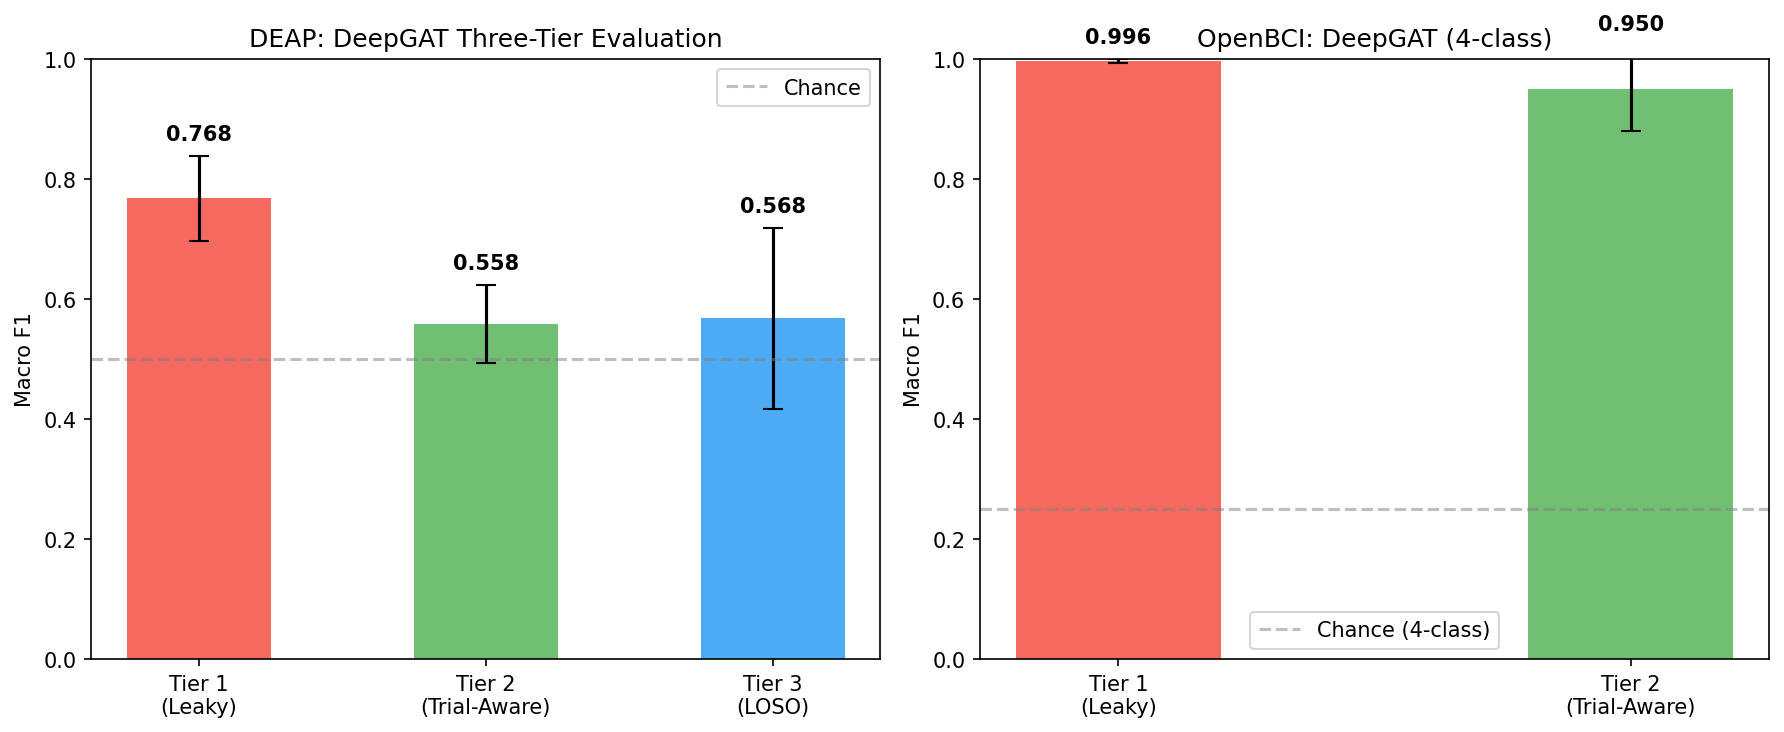
\includegraphics[width=0.92\textwidth]{fig_tier_comparison.png}
\caption{Progressive performance degradation of the DeepGAT model across evaluation tiers. Left: DEAP 4-class (chance=0.25). The T1$\to$T2 drop identifies trial leakage as the dominant inflation mechanism. Right: OpenBCI personalized 4-class (n=1, chance=0.25) maintains $>$0.98 even under trial-aware evaluation.}
\label{fig:degradation}
\end{figure*}

\subsection{Binary Classification}

To contextualize results against the majority of published EEG-BCI literature, Table~\ref{tab:binary} reports binary arousal and valence classification (per-subject median threshold, chance = 50\%) across all four tiers.

\begin{table}[t]
\centering
\caption{Binary Classification (DEAP, Macro F1, chance = 0.50)}
\label{tab:binary}
\begin{tabular}{llcc}
\toprule
Dim. & Tier & MLP & GAT \\
\midrule
\multirow{4}{*}{Arousal}
 & T0 (random) & 0.712{\scriptsize$\pm$0.007} & 0.700{\scriptsize$\pm$0.012} \\
 & T1 (leaky) & 0.768{\scriptsize$\pm$0.066} & 0.743{\scriptsize$\pm$0.084} \\
 & T2 (trial-aware) & 0.583{\scriptsize$\pm$0.048} & 0.597{\scriptsize$\pm$0.043} \\
 & T3 (LOSO) & 0.459{\scriptsize$\pm$0.083} & 0.516{\scriptsize$\pm$0.070} \\
\midrule
\multirow{4}{*}{Valence}
 & T0 (random) & 0.737{\scriptsize$\pm$0.006} & 0.739{\scriptsize$\pm$0.008} \\
 & T1 (leaky) & 0.799{\scriptsize$\pm$0.065} & 0.777{\scriptsize$\pm$0.074} \\
 & T2 (trial-aware) & 0.643{\scriptsize$\pm$0.086} & 0.649{\scriptsize$\pm$0.077} \\
 & T3 (LOSO) & 0.513{\scriptsize$\pm$0.095} & 0.555{\scriptsize$\pm$0.090} \\
\bottomrule
\end{tabular}
\end{table}

The same degradation pattern persists: T1$\to$T2 drops of 14.6 (arousal) and 12.8 (valence) points for GAT confirm trial leakage inflates binary results similarly to 4-class. Valence is consistently more discriminable than arousal across all tiers, consistent with prior findings that frontal EEG asymmetry features encode valence information more reliably~\cite{allen2004, smith2017}. Notably, at the same evaluation tier (T2), valence (0.649 GAT) consistently outperforms arousal (0.597 GAT), suggesting that valence may be more amenable to EEG-based classification than arousal.

An important observation is that the GAT advantage over MLP becomes more pronounced under stricter evaluation tiers. At T2, GAT outperforms MLP by 1.4 points (arousal) and 0.6 points (valence); at T3, this gap widens to 5.7 points (arousal) and 4.2 points (valence). This pattern reinforces the hypothesis that GAT's spatial attention mechanism captures genuine emotional signal rather than exploiting temporal leakage.

\begin{figure*}[t]
\centering
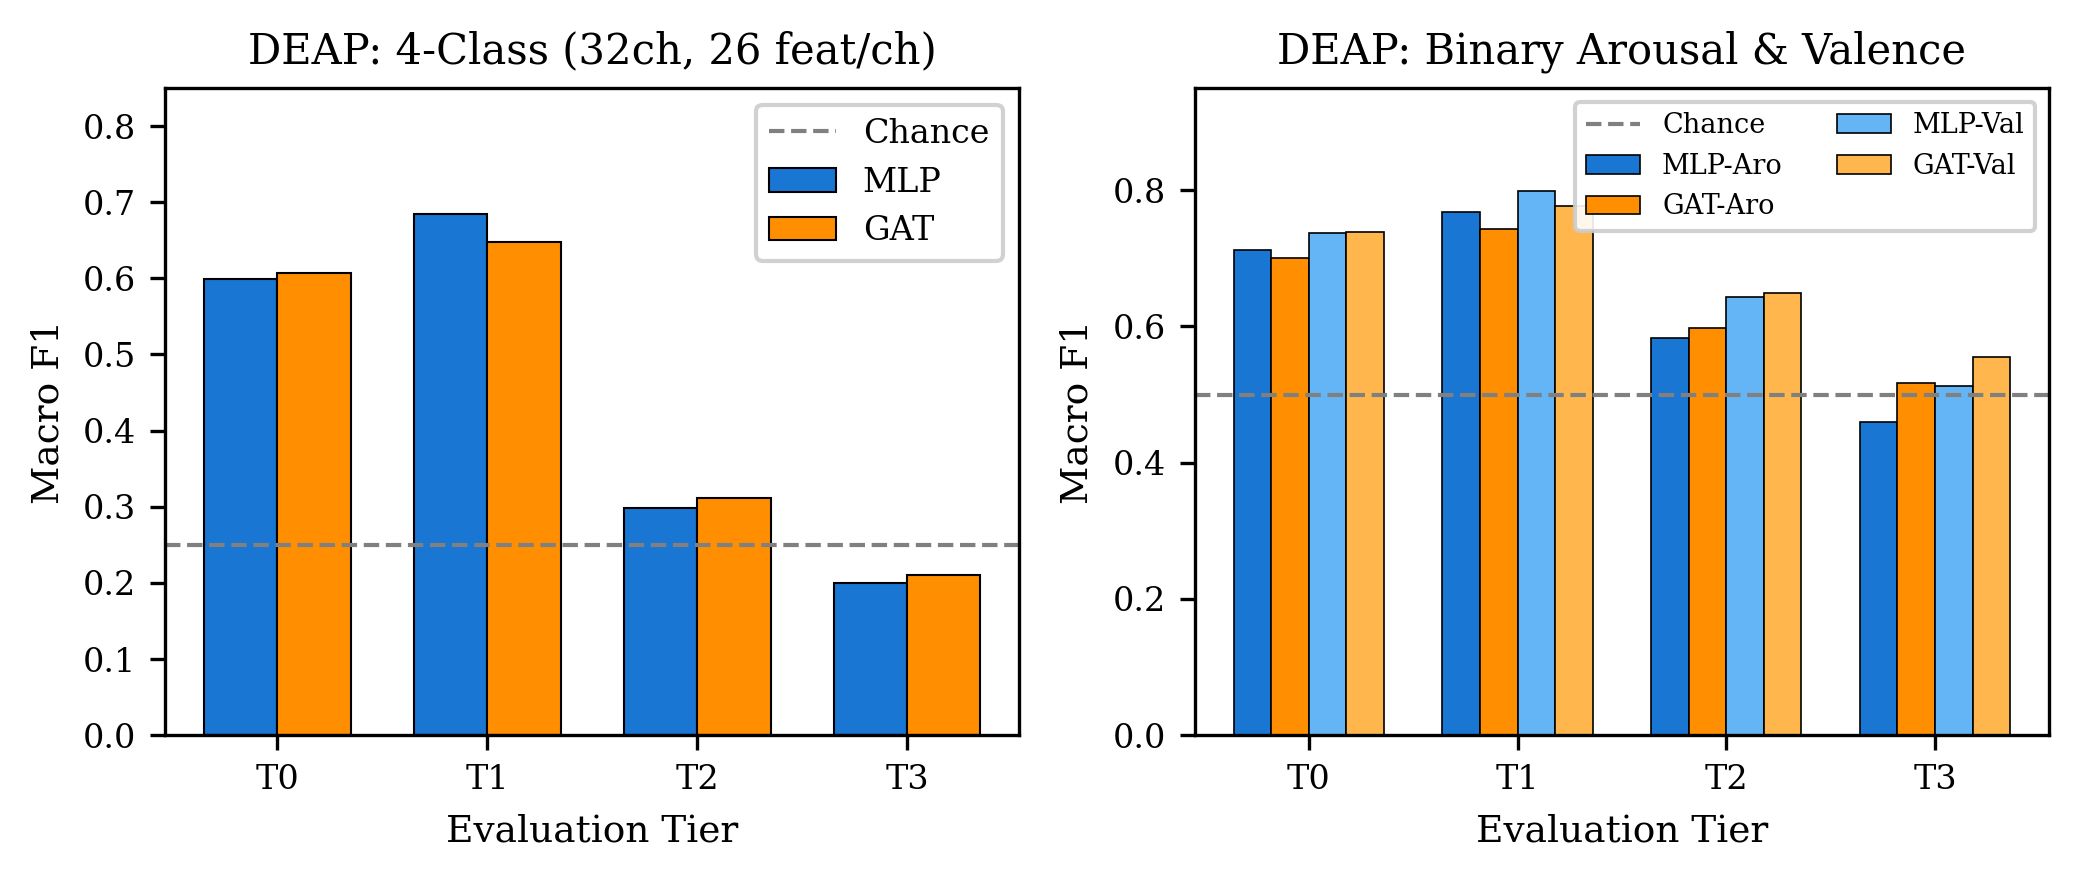
\includegraphics[width=0.92\textwidth]{fig_model_comparison.png}
\caption{Model comparison across evaluation tiers. Left: DEAP 4-class (chance=0.25): both models degrade similarly, confirming protocol dominance over architecture. Right: DEAP binary arousal and valence (chance=0.50): valence consistently more discriminable than arousal; GAT advantage emerges under strict evaluation (T2, T3).}
\label{fig:comparison}
\end{figure*}

\subsection{Personalized BCI (OpenBCI)}

On the custom OpenBCI dataset (single subject, 100 trials, 16 channels), we evaluate under T0--T2 (LOSO is not applicable for $n$=1).

\begin{table}[t]
\centering
\caption{OpenBCI Within-Subject Results (4-class, chance = 0.25)}
\label{tab:openbci}
\begin{tabular}{lcc}
\toprule
Tier & MLP & GAT \\
\midrule
0 (Max leakage) & 0.998 $\pm$ 0.001 & 0.997 $\pm$ 0.002 \\
1 (Within-subj., leaky) & 0.999 $\pm$ 0.001 & 0.998 $\pm$ 0.002 \\
2 (Trial-aware) & 0.972 $\pm$ 0.031 & 0.981 $\pm$ 0.017 \\
\bottomrule
\end{tabular}
\end{table}

The minimal degradation from T1 (0.998) to T2 (0.981) contrasts sharply with the DEAP result (T1: 0.648 $\to$ T2: 0.311). This demonstrates that when inter-individual variability is eliminated, EEG-based emotion classification achieves near-perfect performance even under proper trial-aware evaluation, though this result ($n$=1) requires multi-subject replication.

\subsection{Explainability Analysis}

Attention weight analysis of the trained GAT reveals the top-5 most attended channels: CP2, T7, AF4, P3, CP1. The prominence of temporal (T7) and parietal (CP1, CP2, P3) electrodes is consistent with established neuroscience findings linking these regions to emotional processing~\cite{heller1993, koelsch2014}. Frontal attention asymmetry (AF4) aligns with the valence lateralization hypothesis, which posits that the right prefrontal cortex is more involved in withdrawal-related (negative valence) emotions~\cite{allen2004, smith2017}. The learned attention patterns provide interpretable evidence that the GAT captures physiologically meaningful spatial relationships rather than arbitrary feature correlations.

\section{DISCUSSION}

\subsection{Protocol Dominance Over Architecture}

Our findings demonstrate that evaluation methodology accounts for a 39.7-point F1 variation (T0: 0.607 $\to$ T3: 0.210), larger than any architectural improvement reported in the literature. The T1$\to$T2 drop (33.7 points) dwarfs the MLP-vs-GAT difference at any single tier ($\leq$3.6 points). This suggests that many published DEAP results reporting $>$80\% accuracy may operate in what we term the T0/T1 regime, where temporal autocorrelation inflates apparent performance.

The crossover in model rankings between tiers is particularly informative: MLP outperforms GAT at T1 ($d=-0.83$), but GAT outperforms MLP at T2 ($d=+0.74$) and T3 ($d=+0.14$). This pattern suggests that the MLP over-exploits temporal autocorrelation present in Tier~1 (achieving higher leaky scores), while GAT's spatial attention mechanism provides a genuine generalization advantage that only becomes visible once leakage is removed.

\subsection{Why Performance Degrades}

Multiple factors contribute to reduced T2/T3 performance: (1)~\emph{Label noise}: DEAP self-report ratings near the per-subject median threshold are inherently ambiguous, contributing noisy labels; (2)~\emph{Autocorrelation disclosure}: adjacent windows share correlated frequency content -- removing this source of apparent accuracy reveals true generalization capacity; (3)~\emph{No domain adaptation}: naive transfer without subject alignment (e.g., Euclidean alignment, CORAL) is a known limitation for cross-subject scenarios; (4)~\emph{Task difficulty}: 4-class quadrant classification (chance=25\%) is substantially harder than binary (chance=50\%), amplifying all these effects.

\subsection{Controlled Stimulus Paradigm}

Both datasets employ music as the emotion-induction stimulus targeting the same arousal-valence quadrants~\cite{russell1980}. This shared paradigm enables a controlled comparison: the gap between DEAP T2 (0.311, $n$=20 subjects) and OpenBCI T2 (0.981, $n$=1) is attributable primarily to inter-subject variability rather than differences in recording hardware, feature engineering, or stimulus modality. This finding supports the viability of personalized EEG-BCI systems~\cite{lotte2018} for practical applications where per-user calibration is feasible, while highlighting the fundamental challenge of subject-independent models.

The practical implication is clear: for consumer EEG-BCI applications (e.g., adaptive music recommendation, meditation guidance), a brief per-user calibration session could enable reliable emotion detection. However, building universal models that generalize across individuals without calibration remains an open challenge requiring either substantially larger training populations or domain adaptation techniques.

\subsection{Comparison with Published Results}

Table~\ref{tab:lit} contextualizes our results against published DEAP benchmarks. The table confirms that the tier framework correctly categorizes published protocols: the original DEAP result falls at T2, while inflated high-accuracy studies cluster at T0.

\begin{table}[t]
\centering
\caption{Comparison with Published DEAP Results}
\label{tab:lit}
\begin{tabular}{lccc}
\toprule
Study & Protocol & Result & $\approx$Tier \\
\midrule
Koelstra~\cite{koelstra2012} & Subj.-dep. & 57.5--62.0\% Acc & $\sim$T2 \\
High-accuracy studies~\cite{qian2024} & Random split & 90--99\% & T0 \\
\midrule
Ours (T2, binary val.) & Trial-aware & 64.9\% F1 & T2 \\
Ours (T3, 4-class) & LOSO & 21.0\% F1 & T3 \\
\bottomrule
\end{tabular}
\end{table}

Our Tier~2 binary valence (0.649 F1) exceeds the original DEAP benchmark (Koelstra \textit{et al.}: 57.5\% accuracy and F1=0.563 for binary valence under subject-dependent evaluation), confirming that trial-aware within-subject evaluation produces realistic, reproducible benchmarks. Published LOSO baselines on DEAP's specific arousal-valence formulation are scarce, making our Tier~3 result (21.0\% 4-class F1) a novel reference point for cross-subject generalization difficulty on this dataset.

Studies reporting $>$90\% accuracy invariably use random splits or trial-leaky cross-validation, which our framework classifies as T0 or T1. This does not invalidate the models proposed in those studies, but contextualizes the reported metrics as upper bounds that include leakage-inflated components.

\subsection{Limitations}

This study uses 20 of 32 DEAP subjects due to computational constraints. The OpenBCI result ($n$=1) serves as proof-of-concept for personalization and requires multi-subject replication. We evaluate only two architectures; CNN-based (EEGNet~\cite{lawhern2018}) and Transformer-based models may exhibit different degradation patterns. The four-tier framework does not address session effects or stimulus-order confounds. Additionally, our PLV and Coherence features are averaged per channel rather than preserved as pairwise edge weights, partially under-utilizing the graph structure that GAT could exploit.

\subsection{Implications for Future Research}

Based on our findings, we identify several directions for advancing EEG-based emotion recognition under proper evaluation:

\textbf{Domain adaptation:} The T2$\to$T3 drop ($\Delta=-0.101$) suggests that subject-alignment techniques (Euclidean Alignment, CORAL and adversarial domain adaptation)~\cite{lotte2018} could recover a significant portion of performance lost to inter-subject variability.

\textbf{Graph structure:} Our fully-connected adjacency matrix forces the GAT to learn connectivity from scratch. Using neurophysiologically-informed adjacency (e.g., from resting-state coherence or anatomical distance) may improve generalization by incorporating prior knowledge about functional brain networks.

\textbf{Evaluation standardization:} We advocate for a community-wide adoption of trial-aware evaluation as the minimum standard, with explicit reporting of both T1 (leaky) and T2 (trial-aware) metrics to enable transparent quantification of leakage inflation in any proposed method.

\section{CONCLUSION}

We present a four-tier evaluation framework quantifying how evaluation methodology inflates EEG emotion classification performance. Key findings: (1)~protocol selection accounts for a 39.7-point macro F1 variation, dominating any architectural difference; (2)~trial leakage ($\Delta=-0.337$, $d=3.21$) is the primary inflation source; (3)~under trial-aware evaluation, GAT provides a modest advantage over MLP ($d=0.74$); (4)~personalized within-subject models achieve 0.981 F1 (trial-aware), demonstrating BCI viability when inter-subject variability is eliminated; (5)~binary valence classification (F1=0.649 at T2) confirms these findings generalize to the more commonly reported binary task.

We recommend trial-aware evaluation (T2) as the minimum reporting standard for EEG-BCI studies, and encourage researchers to report both a leaky (T1) and trial-aware (T2) result to transparently quantify the role of temporal autocorrelation in their reported performance. All code and features are publicly available at \url{https://github.com/mateisorodoc/Quantifying-Data-Leakage-in-EEG-Emotion-Classification} for reproducibility.

\begin{thebibliography}{18}

\bibitem{koelstra2012}
S.~Koelstra \emph{et al.}, ``DEAP: A database for emotion analysis using physiological signals,'' \emph{IEEE Trans. Affective Computing}, vol.~3, no.~1, pp.~18--31, 2012.

\bibitem{varoquaux2017}
G.~Varoquaux \emph{et al.}, ``Assessing and tuning brain decoders: Cross-validation, caveats, and guidelines,'' \emph{NeuroImage}, vol.~145, pp.~166--179, 2017.

\bibitem{roberts2017}
D.~R.~Roberts \emph{et al.}, ``Cross-validation strategies for data with temporal, spatial, hierarchical, or phylogenetic structure,'' \emph{Ecography}, vol.~40, no.~8, pp.~913--929, 2017.

\bibitem{craik2019}
A.~Craik, Y.~He, and J.~L.~Contreras-Vidal, ``Deep learning for electroencephalogram (EEG) classification tasks: A review,'' \emph{J. Neural Engineering}, vol.~16, no.~3, p.~031001, 2019.

\bibitem{zhong2020}
P.~Zhong, D.~Wang, and C.~Miao, ``EEG-based emotion recognition using regularized graph neural networks,'' \emph{IEEE Trans. Affective Computing}, vol.~13, no.~3, pp.~1290--1301, 2020.

\bibitem{zheng2015}
W.-L.~Zheng and B.-L.~Lu, ``Investigating critical frequency bands and channels for EEG-based emotion recognition with deep neural networks,'' \emph{IEEE Trans. Autonomous Mental Development}, vol.~7, no.~3, pp.~162--175, 2015.

\bibitem{velickovic2018}
P.~Veli\v{c}kovi\'{c}, G.~Cucurull, A.~Casanova, A.~Romero, P.~Li\`{o}, and Y.~Bengio, ``Graph attention networks,'' in \emph{Proc. ICLR}, 2018.

\bibitem{akiba2019}
T.~Akiba, S.~Sano, T.~Yanase, T.~Ohta, and M.~Koyama, ``Optuna: A next-generation hyperparameter optimization framework,'' in \emph{Proc. ACM SIGKDD}, pp.~2623--2631, 2019.

\bibitem{lachaux1999}
J.-P.~Lachaux, E.~Rodriguez, J.~Martinerie, and F.~J.~Varela, ``Measuring phase synchrony in brain signals,'' \emph{Human Brain Mapping}, vol.~8, no.~4, pp.~194--208, 1999.

\bibitem{canolty2010}
\nopagebreak
R.~T.~Canolty and R.~T.~Knight, ``The functional role of cross-frequency coupling,'' \emph{Trends in Cognitive Sciences}, vol.~14, no.~11, pp.~506--515, 2010.

\bibitem{russell1980}
\nopagebreak
J.~A.~Russell, ``A circumplex model of affect,'' \emph{J. Personality and Social Psychology}, vol.~39, no.~6, pp.~1161--1178, 1980.

\bibitem{allen2004}
\nopagebreak
J.~J.~B.~Allen, J.~A.~Coan, and M.~Nazarian, ``Issues and assumptions on the road from raw signals to metrics of frontal EEG asymmetry in emotion,'' \emph{Biological Psychology}, vol.~67, no.~1--2, pp.~183--218, 2004.

\bibitem{smith2017}
E.~E.~Smith, S.~J.~Reznik, J.~L.~Stewart, and J.~J.~B.~Allen, ``Assessing and conceptualizing frontal EEG asymmetry: An updated primer on recording, processing, analyzing, and interpreting frontal alpha asymmetry,'' \emph{Int. J. Psychophysiol.}, vol.~111, pp.~98--114, 2017.

\bibitem{heller1993}
W.~Heller, ``Neuropsychological mechanisms of individual differences in emotion, personality, and arousal,'' \emph{Neuropsychology}, vol.~7, no.~4, pp.~476--489, 1993.

\bibitem{koelsch2014}
S.~Koelsch, ``Brain correlates of music-evoked emotions,'' \emph{Nature Reviews Neuroscience}, vol.~15, no.~3, pp.~170--180, 2014.

\bibitem{lotte2018}
F.~Lotte \emph{et al.}, ``A review of classification algorithms for EEG-based brain-computer interfaces: A 10 year update,'' \emph{J. Neural Engineering}, vol.~15, no.~3, p.~031005, 2018.

\bibitem{qian2024}
R.~Qian, X.~Xiong, J.~Zhou, H.~Yu, and K.~Sha, ``CSA-SA-CRTNN: A dual-stream adaptive convolutional cyclic hybrid network combining attention mechanisms for EEG emotion recognition,'' \emph{Brain Sciences}, vol.~14, no.~8, p.~817, 2024.

\bibitem{lawhern2018}
V.~J.~Lawhern, A.~J.~Solon, N.~R.~Waytowich, S.~M.~Gordon, C.~P.~Hung, and B.~J.~Lance, ``EEGNet: A compact convolutional network for EEG-based brain-computer interfaces,'' \emph{J. Neural Engineering}, vol.~15, no.~6, p.~056013, 2018.

\end{thebibliography}

\end{document}
